\begin{comment}
2.2 Teil I: Bericht
Problemstellung, Ziele, Einführung, Einleitung
Warum machen wir das Projekt? Wieso haben wir dieses Projekt bearbeitet?
2.2.2 Aufgabenstellung
Welche Ziele wurden gesteckt (Kann-Ziele, Muss-Ziele)
Die vom Betreuer abgegebene und unterschriebene Aufgabenstellung.
Bei Fortsetzungsarbeiten geht der Aufgabenstellung eine tabellarische Aufstellung voran (Einleitung), welche klar aufzeigt, was während der ersten Arbeit wurde.
2.2.3 Rahmenbedingungen
Meist vorgegeben.
2.2.4 Vorgehen, Aufbau der Arbeit
Vorgehen: Was wurde gemacht? In welchen Teilschritten? Risiken der Arbeit? Wer war involviert (Durchführung, Entscheide usw.)? Details in anderen Kapiteln.
Einführung in die Problem- und Aufgabenstellung. Übersicht über die übrigen Teile der Abgabe.
2.2.5 "Stand der Technik"
Zweck und Inhalt dieses Kapitels.
Was machen andere / welche ähnlichen Arbeiten gibt es zum Thema? Was kann von anderen verwendet werden?
Diese Einleitung soll für den Ingenieur irgendeiner Fachrichtung verständlich sein. Sie stellt die Aufgabe in einen grösseren Zusammenhang und liefert eine genaue Beschreibung der Problemstellung. Allfällige Vorarbeiten oder ähnlich gelagerte Arbeiten werden diskutiert.
Theoretische Grundlagen sind nur so weit auszuarbeiten, als dies für die Lösung der Aufgabe nötig ist (keine Lehrbücher schreiben). Die Erkenntnisse aus den theoretischen Untersuchungen sind wenn immer möglich direkt mit der Problemlösung zu verknüpfen.
2.2.6 Bewertung (Evaluation)
Evaluieren heisst Bewerten. Objektives Bewerten geschieht immer über Kriterien, qualitative (evtl. quantifiziert) und quantitative.
2.2.7 Vision, Umsetzungskonzept
Da drin steckt den Kern der Lösungsidee und des Konzeptes.
2.2.8 Resultate: Bewertung und Zielerreichung
Bewertung der Resultate. Vergleich mit anderen Lösungen.
Was ist Neuartig an der Arbeit? Was ist der Nutzen der Arbeit (quantifizierbar/nicht quantifizierbar)? Was sind die (externen) Kosten der Arbeit?
Zielerreichung: was wurde erreicht, was wurde nicht erreicht bezüglich Kann-/Muss-Zielen? Abweichungen (positiv und negativ) und kurze Begründung dafür.
2.2.9 Schlussfolgerungen und Ausblick
Die Schlussfolgerungen bilden zusammen mit der Zusammenfassung die wichtigsten Abschnitte eines Berichts und sollen daher am sorgfältigsten ausgearbeitet sein. Die Schlussfolgerungen enthalten eine Zusammenfassung und Beurteilung der Resultate (Vergleich mit anderen Lösungen, was wurde erreicht, was nicht, was bleibt noch zu tun, was würde man nun anders tun).
In den Schlussfolgerungen soll auch ein Ausblick auf das weitere Vorgehen bzw. auf die Bedeutung der erreichten Ergebnisse gegeben werden.
Weiteres zum Ausblick siehe Kapitel 2.3.9 Weiterentwicklung.
2.2.10 Persönliche Berichte und Dank (fakultativ)
Persönlicher Bericht der Studierenden zu ihren Erfahrungen bei der Arbeit. Bei Vorträgen ein sicher interessanter Teil; in der Diplomarbeit je nach dem.
\end{comment}


\part{Technischer Bericht}
\glsresetall


\chapter{Einführung}

\section{Vision}


\section{Ziele}


\section{Rahmenbedingungen}
\section{Kommunikation}
Bei der Durchführung der Bachelorarbeit DAT wollten wir auf die Kommunikation per E-Mail verzichten. Wir haben unsere Informationen zwischen Mitarbeitern und Dozenten, wie zur Protokollierung der Sitzungen mittels \hyperlink{http://www.slack.com}{Slack} ausgetauscht. Slack bietet Team-Kommunikation auf hohem Niveau, mit der Möglichkeit Services wie GitHub oder Travis zu integrieren. So konnte an einem Zentralen Ort Bezug auf Commits und Build Results genommen werden. Durch die Verwendung eines dedizierten Tools zur Kommunikation konnte das E-Mail Postfach von Bachelor relevanten Themen frei gehalten werden und direkt Bezug auf konkrete Ereignisse genommen werden. \\
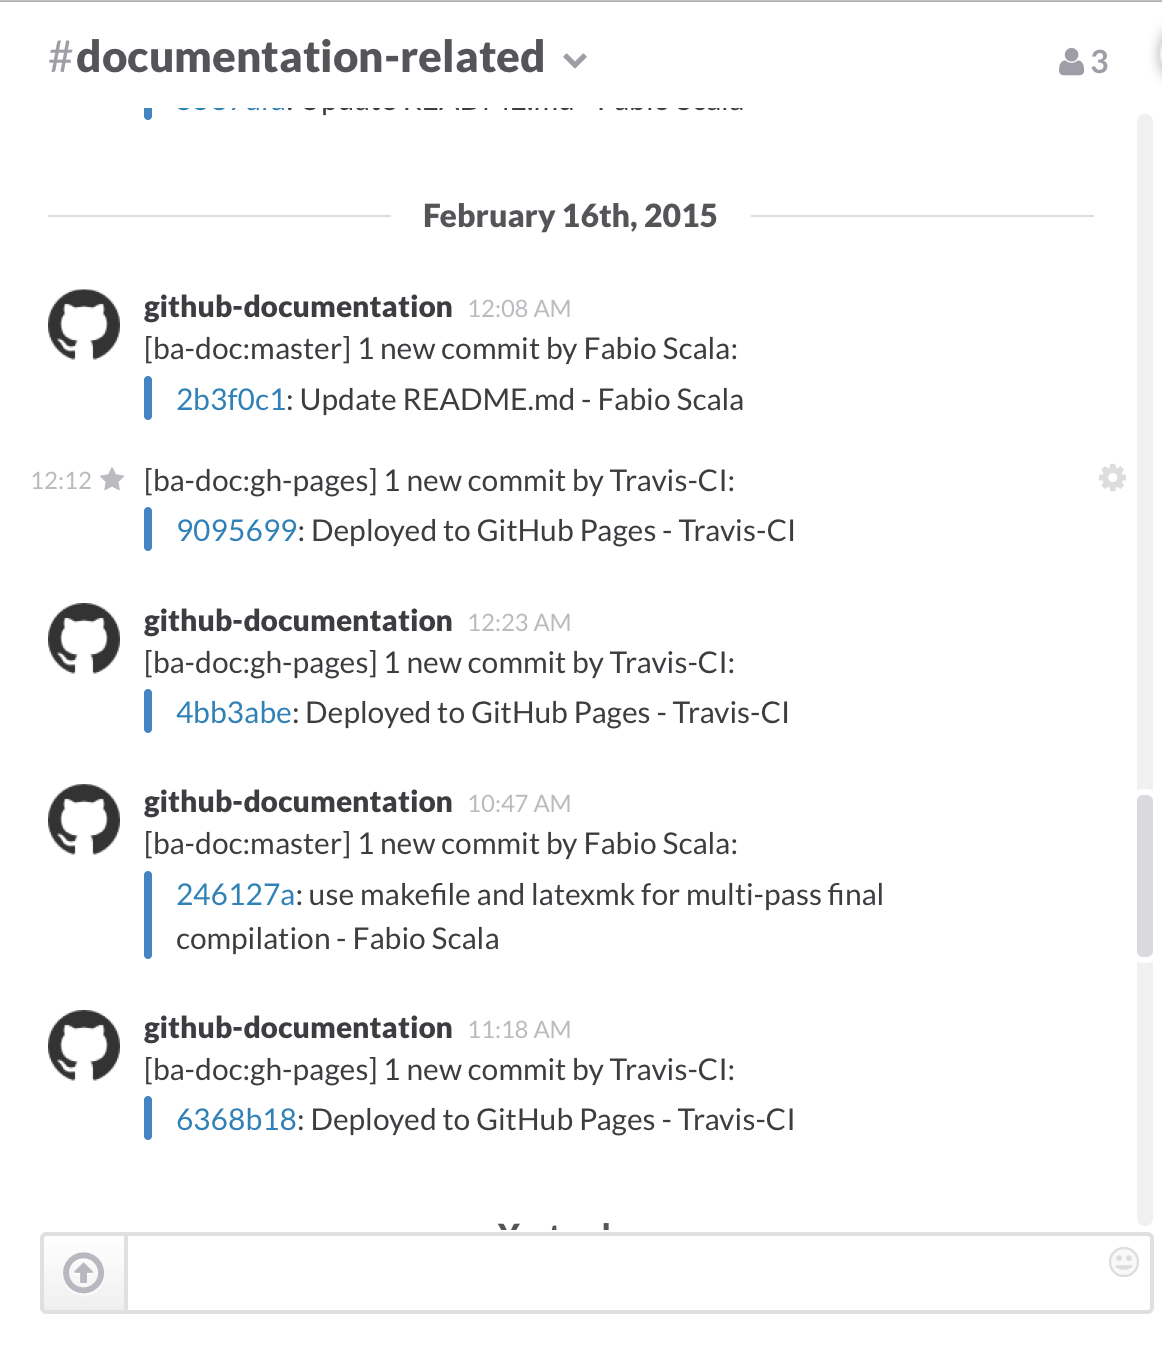
\includegraphics[scale=0.5]{slack.png}


\chapter{Umsetzung}

\section{Stand der Technik}


\chapter{Resultate und Ausblick}


\section{Persönlicher Bericht}


\section{Dank}


